\documentclass[a4paper,11pt]{kth-mag}
\usepackage[T1]{fontenc}
\usepackage{textcomp}
\usepackage{lmodern}
\usepackage{amsmath}
\usepackage[swedish,english]{babel}
\usepackage{modifications}
\usepackage[usenames,dvipsnames,svgnames,table]{xcolor}
\usepackage[toc]{glossaries}
\usepackage{pgfplots}
\usepackage{graphicx}
\usepackage{pgfplotstable}

\graphicspath{ {img/} }
\pgfplotsset{width=12cm,compat=1.9}

\newglossaryentry{computer}{
  name=computer,
  description=
  {is a programmable machine that receives input,
    stores and manipulates data, and provides
    output in a useful format}
}
\newglossaryentry{MLE}{
  name=Maximum Likelihood Estimate,
  description=
  {\todo yolo}
}
\newglossaryentry{BFS}{
  name=Breadth First Search,
  description={Basic search algorithm where each previously unexamined connecting neighbor of a node is examined in a iteration, and the queued to be subject for the next iteration.}
}
\newglossaryentry{wordnet}{
  name=WordNet,
  description={WordNet\cite{wordnet} is a lexical database for English. WordNet has nouns, verbs, adjectives and adverbs grouped into sets of cognitive synonyms (synsets), each expressing a distinct concept. These synsets are interlinked by means of conceptual-semantic and lexical relations.}
}
\newglossaryentry{jaws}{
  name=JAWS,
  description={JAWS\cite{jaws} is a library providing API methods for accessing synset relations in \gls{wordnet}}
}

\newglossaryentry{superword}{
  name=hypernym,
  description={A word relation implying less specific meaning. For example, \emph{color} is a hypernym of \emph{red}.}
}



\newcommand{\todo}{ ... }
\newcommand{\ngram}{$n$-gram}
\newcommand{\category}{restaurant category }  % may become plural
\newcommand{\numAnnotated}{12}
\newcommand{\numClassifierAproaches}{2}
\newcommand{\numClassifiationReviews}{2}

\newif\ifhasStudiedFailures
\hasStudiedFailuresfalse

\newcommand{\loremipsum}{
  {\color{lightgray}
  Fruit two greater fifth over every. In female fourth good wherein herb
  Waters yielding itself. Female greater. Hath in, second appear tree in.
  Him, it seasons. Upon. Good you're. Winged green. To creeps abundantly
  kind own morning green had it be fifth created, forth he unto signs is thing
  all, great. Place night Gathering upon were forth light deep. Abundantly.
  Kind air beginning his void seed it dry. Own and spirit may dry abundantly
  beast good forth. The fifth beginning. Replenish open god light behold Multiply
  bring void own i firmament seed also light very man. \gls{computer}

  }
}

\makeglossaries

\title{Something, something, something, thesis...}

\subtitle{Getting a degree is hard}
\foreigntitle{Getting a degree is hard in swedish too}
\author{Mattis Kancans Envall}
\date{June 2016}
\blurb{Master's Thesis at CSC\\Supervisor: Johan Boye\\Examiner: Viggo Kann}
\trita{TRITA xxx yyyy-nn}


\begin{document}
\frontmatter
\pagestyle{empty}
\removepagenumbers
\maketitle
\selectlanguage{english}
\begin{abstract}
  This is a skeleton for KTH theses. More documentation
  regarding the KTH thesis class file can be found in
  the package documentation.

\loremipsum

\end{abstract}
\clearpage
\begin{foreignabstract}{swedish}
\loremipsum

\end{foreignabstract}
\clearpage
\tableofcontents*

\glsaddall
\printglossaries

\mainmatter
\pagestyle{newchap}
\chapter{Introduction}
With increased internet usage, reviews online are becoming one of the most important resources when comparing businesses, services and products.
The increasing quantity of content makes for more reliable conclusions as more opinions can be taken into account, but it also poses a problem,
since there is a limit to what human readers can process.

Computers are obviously faster and more capable to handle big quantities of data, which suggests potential for using computers as aid when
interpreting review-like content. This is studied under the name \emph{Sentiment Analysis}, and has been in very active research the last ten years
thanks to increases in available data and recent efforts to monetize it.

This degree project studies describes sentiment analysis with regard to mining and summarizing opinions in reviews, and provides a detailed study of some of the problems in this process; identifying opinions, classifying their sentiment, and categorizing what the opinion to enable summarization.

It is layed out the following way: First there is a common introductory section with shared background for all of the three \todo


%This general problem is called \emph{sentiment analysis}\cite{liu2012sentiment} and is widely considered a hard, non-trivial problem.
%sentiment analysis is one of the most active fiels of research in NLP.

%The general problem of using computers and Natural Language Processing(NLP)-techniques to study opinions in text s called \emph{sentiment analysis}, and is one of the most active fields of study in NLP.

%In fact, recent trends of monetizing online content, not to mention the benefit of being able to

\section{Sentiment analysis}
Sentiment analysis\cite{liu2012sentiment} is the general task of from raw text extracting and interpreting expressions with associated sentiments. This involves classifying orientation (and possibly intensity) of found sentiments, and identifying what entity, and possibly what aspect of that entity, is subject to the expressed sentiments.

\subsection{Levels of sentiment analysis}
In general, sentiment analysis has been studied at three levels:

On the \emph{document level}, one overall sentiment of an entire document is identified. This is generally of limited use, as in most contexts, documents hold many opinions. Therefore most studies at the document level in some way handle conflicting opinions, although this may be done implicitly\cite[Chapter~3]{liu2012sentiment}. In document level sentiment analysis, the problem definition itself requires generalizations, which may invite to inaccurate over-simplifications.

\emph{Sentence level} sentiment analysis mitigates this risk of generalization; sentences are generally smaller than documents and thus less likely to hold conflicting opinions, so assuming there is at most one sentiment has less impact on results --- but the problem itself is not addressed. As an example, the sentence \emph{``Although the service is terrible, I still like this restaurant''} is arguably overall positive, but simply deeming it so excludes information which reduces quality of results and makes them susceptible to systematic errors.

%todo examples in table?
Ideally two opinions should be identified in the above sentence, one about \emph{service} and one about the reviewed entity in general. Sentiment analysis this fine grained is on the \emph{aspect level}. The goal is to find and classify individual opinions, which may  dealing with things like surjective opinions \emph{``food, service and ambiance were all great''}, conjunctions \emph{``tasty but expensive''}, implicit references \emph{``Easy to fit in my pocket''} really implies \emph{``good size''}, and implicit references \emph{``I had pasta. It was great''}'. As such, sentiment analysis on the aspect level is commonly referred to as the most complicated, as it consists of several sub-problems\cite[chapter 1]{liu2012sentiment}.


\section{Important definitions}

\subsubsection{Opinion}
\emph{Liu} (2012) introduces the opinions as $(e_i,a_{ij},s_{ijkl},h_k,t_l)$-quintuples\footnote{Subscripts are used to indicate dependencies between tuple elements.}, where $e_i$ is the entity the opinion is referencing, $a_{ij}$ is the aspect of $e_i$ that is being referenced (e.g. for a restaurant its ambience), $s_{ijkl}$ is the sentiment of the opinion, $h_k$ is the opinion holder and $t_l$ is the time of the experience the opinion is based on\cite[Chapter~2.1]{liu2012sentiment}.

In this work, Yelp reviews are used, and a few assumptions will make to simplify:
\begin{itemize}
\item The opnion holder $h_k$ is the user posting the review.
\item The time $t_l$ is the time of the review.
\item The entity $e_i$ being reviewed is the business for which the review is being posted.
\end{itemize}

%todo discuss assumption consequences?
Thus in this report, an opinion can generally be thought of as a $(a,s)$ tuple.
% aspects are also synonymously referred to as \emph{opinion targets}.

\subsubsection{Word}
The term ``word'' can be a bit ambigous and need a more specific definion of usage. In this report it is used to reference what is also known as \emph{word form}. That is, one specific alphabetical representation of a lemma, which can have more than one representation.

\subsubsection{Word sense}
%A few terms in linguistics are rather ambiguous and require definitions of usage. In this report it is used synonymously with the term \emph{lemma}, as defined by D. Jurafsky and J.H. Martin\cite{nlpbook}. Similarly, the definition of \emph{word sense} from the same source will be used to reference single meaning of a word; e.g. \textbf{bank$^1$} (``financial institution'') and \textbf{bank$^2$} (``sloping mound'') are different \emph{word senses} even though they share one \emph{word form}.

\section{Language modeling}

\subsection{\ngram s}
\ngram~modeling is a versatile, robust and widely used method of modeling languages. Typically the model consists of, for some $n$, all $n$-length sub-sequences of a longer sequence (i.e. one or many documents). Each unique sub-sequence is then referred to as a \ngram, and \ngram s of length \emph{1,2,3} are referred to as \emph{unigrams, bigrams} and \emph{trigrams}, respectively\cite{ngrams}.

Frequencies, counts and occurrences of \ngram s have been used in language modeling\cite{chen_goodman}, text categorization\cite{ngrams}, \todo

As an example, the word-\emph{bigrams} for the sentence \emph{``Languages are fun''} are:
\begin{quote}
  \vspace*{0.1cm}
  \centering
\emph{``\$ Languages''}, \emph{``Languages are''}, \emph{``are fun''}, and \emph{``fun \$''}
\end{quote}
where \emph{\$} is a token meaning the start/end of sentence.

Although \ngram~modeling can be applied to virtually any kind of sequence, this report henceforth will refer exclusively to \ngram s consisting of words.

\newpage
\subsection{\ngram~ language modeling}
If the probability of a word's occurrence in a sentence $P$ is known (e.g. estimated using a corpus), then the probability of a sentence $s$ can be modeled the following way with \emph{unigrams}:

\begin{equation} \label{eq:unigram_chain_prob}
P(s) = P(w_1) P(w_2) \dots P(w_n) =\prod_{w_i \in s}P(w_i)
\end{equation}
or similarly, if modeled with \emph{bigrams} based on the Markov assumption (the probability of a word's occurrence only depends on previous word(s) in the sentence):

\begin{equation} \label{eq:bigram_chain_prob}
P(s) = P(w_2 | w_1)P\times (w_3 | w_2) \times \dots \times P(w_n | w_{n-1}) = \prod_{w_i \in s}P(w_i|w_{i-1})
\end{equation}
Where $P(w_b | w_a)$ is some probability estimate of a word being $w_b$ provided that the previous word was $w_a$. It should be clear that good \ngram~modeling then is about finding a $P$-function that estimates reality well.

A naive \gls{MLE} of a sentence $s$ could be defined something like this:
\begin{equation} \label{eq:bigram_mle}
P(w_i|w_{i-1}) = \frac{c(w_{i-1}\,w_i)}{\sum_{w} c(w_{i-1}\, w)}
\end{equation}

Here the number of occurrences where the word $w_{i-1}$ follows $w_i$ (as provided by the count function $c$) are normalized by the number of occurrences where $w_{i-1}$ is followed by any word $w$, or in other words the fraction of this particular bigram out of all bigrams with the same first word.

\subsection{Smoothing language models}
A general problem when statistically modeling based on existing data, is how the model should handle previously unseen entities. Since human language is virtually infinite, even reasonable sentences are innumerable, and thus that is a requirement for good performance.

As can be seen in equation \ref{eq:bigram_mle}, this would per definition assign a zero probability to entities unseen in training data, which in turn makes the \gls{MLE} model(eq.~\ref{eq:bigram_chain_prob}) assign a zero probability to the entire sentence\cite{chen_goodman}.

Smoothing is a means of improving this. One of the most basic smoothing techniques called \emph{Lidstone Smoothing} or \emph{additive smoothing} addresses this by introducing a constant $\alpha$ that ensures non-zero probabilities\cite{chen_goodman}:
\begin{equation} \label{eq:additive_smoothing}
P_{add}(w_i|w_{i-1}) = \frac{c(w_{i-1}\,w_i)+\alpha}{\sum_{w} \big[c(w_{i-1}\, w)\cdot\alpha\big]}
\end{equation}
where $0 < \alpha \leq 1$ is commonly used.

\section{Classification methods}
The previous section introduces language modeling, which is used to give the probability of a sentence. Classification can fairly simply be reduced to language modeling, by training one model per class and selecting the model assigning the highest probability. This is in fact what many famous classifiers do. (In fact, eq. \ref {eq:bigram_mle} could be interpreted as a Naive Bayes classifier with only one class(prior=1), and \ngram~occurencies are assumed independent.)

\subsection{Scikit-learn and other classification methods}
Scikit-learn\cite{scikit-learn} is a colleciton of machine learning tools, ready to use ``out of the box''.


\section{Evaluation}
A common way to evaluate information retrieval tasks is \emph{precision} and \emph{recall}. Together they evaluate a systems quality, by evaluating the capacity to exclude irrelevant results, and include relevant results, respectively.

\subsection{Precision}
Precision is a measure of what fraction of retrieved results are considered relevant, see individual parts for exact definitions.

It is defined as following:
\begin{equation} \label{eq:precision}
Precision = \frac{\text {true positives}}{\text{true positives} + \text{false positives}}
\end{equation}
%From this definition it should be clear that precision can by excluding uncertain items from retrieved results.

\subsection{Recall}
Similarly, recall is the fraction of relevant results that are retrieved:
$$Recall = \frac{\text {true positives}}{\text{true positives} + \text{false negatives}}$$
The reader may note from these definitions that more hesitance when including results would mean fewer false positives, but more false negatives, which implies that higher precision can be achieved at the cost of lower recall; or in other words that there is a trade-off between precision and recall to be made.


\subsection{Skewed data}
\label{subsec:bias}
When dealing with real world data, it is also very possible that some classes in classification problems are more common than others. This has been shown to have consequences both in Bayesian classifiers\cite{rennie2003bias} and Support Vector Machines\cite{svm_bias}, where both have been shown to favor majority classes\cite{rennie2003bias, svm_bias}.

Not only classification methods, but also precision measures are affected by skewed data. In binary classification with evenly distributed classes, a classifier that favors one class to the extreme that it always chooses the same class, still achieves around 0.5 precision since the number of true positives would equal the proportion of the favored class\footnote{This is in fact be the worst possible result in the binary case, since any classifier performing consistently worse could be modified to return the opposite and thus have the inverse precision.}. This also illustrates that there is a dependency between precision of biased classifiers and distribution of classes in test data.

A commonly employed and simple way to solve problems with disproportionate data altogether is to exclude all but an equal amount from each class to artificially balance the class distribution, also sometimes referred to as \emph{down-sampling}\cite{provost2000machine}. This could pose a problem if data is very skewed, as this means that the required amount of data is effectively multiplied by the fraction of the least common class. However, in this work the data was not skewed enough to consider more sophisticated other approaches.

Although artificially balanced evaluation data eliminates bias in evaluations, which makes evaluations between classifiers more comparable, it also reduces the amount of entries used for evaluation, which makes evaluations less informed. Therefore this repport will evaluate unscaled data once classifiers have been verified to be reasonably unbiased in a per class comparison.


\part{Sentiment Classification}
\chapter{Sentiment Classification}
Sentiment classification is the problem of deciding whether sentiment in a sentence is positive, negative or neutral\cite{nlp_book}. Being a central part of sentiment analysis it can also done on the same three levels: Document level, sentence level and aspect level.

Sentiment classification can be a classification- or regression analysis problem\cite{liu2012sentiment}, depending on whether results are expected to be discrete class-labels or a continuous measures of positively. In this report the discrete classification definition will be used unless otherwise specified.

Various approaches to sentiment classification exist, where approaches can generally be categorized as either grammatical\cite{todo}, statistical\cite{todo}, or various combinations of the two.




\subsection{Back-off smoothing}

\subsection{Yelp's sentiment analyzer}



\section{Related work}

\subsubsection{Turney (2002)}
In early work, Peter Turney classified sentiment of reviews for automobiles, banks, movies and travel destinations with ranging from 66-84\%, by extracting aspects using predefined POS-patterns, and querying search engines for the co-occurence between found patterns and the words \emph{``excellent''} and \emph{``poor''}.


\subsubsection{Hu, Liu (2004)}
In ``Mining Opinion Features in Customer Reviews'', reviews are  POS-tagged and common data mining methods are used to on to extract features(aspects).

\subsubsection{Hu, Liu (2004)}
In ``Mining and summarizing customer reviews'', their previous work is extended with sentiment classification to produce product summaries. Sentiment is classified by looking for sentiment words predefined as positive or negative or their synonys/antomyms using WordNet. Their method also searches for nearby \emph{negation words}, which if found, simply negate the outcome of the classification.

Finally a summary is produced, but this is very breifly described, and no evaluations of this process are provided.


\section{Experiment setup}
\numClassifiationReviews~reviews, half positive(rated 5/5) and half negative(rated 1/5), were randomly selected from all business categories. Based on the assumption that positive reviews predominantly more positive language than negative reviews, review sentences were labeled according to their review rating. These reviews were then divided into two equal parts, one training set and one testing set, both with equal parts positive and negative Reeves.



\section{Results}



\subsection{Introducing confidence thresholds}
\begin{figure}[h]
  %numpos 3216 numneg 1271
  \centering
  \begin{tikzpicture}
    \begin{axis}[
        xlabel={Recall},
        ylabel={Precision},
        %xmin=0.5, xmax=1,
        %ymin=0.4, ymax=1,
        %xtick={0,20,40,60,80,100},
        %ytick={0,20,40,60,80,100,120},
        legend pos=south west,
        ymajorgrids=true,
        grid style=dashed,
      ]
      \addplot table [x=r, y=p]{data/sent_yelp_pr.csv};
      \addplot table [x=r, y=p]{data/sent_unigram_pr.csv};
      \addplot table [x=r, y=p]{data/sent_bigram_pr.csv};
      \legend{
        Modifier Kneyser-Rey,
        Unigram ensemble,
        Bigram ensamble,
      }
    \end{axis}
  \end{tikzpicture}
  \caption{Sentiment analyzers' precision vs. recall}
  \label{fig:pr_curve}
\end{figure}


\section{Discussion}

% logical negation might clash with bi-gram model



\chapter{Aspect extraction}

The previous parts of this work have introduced methodology to extract

\section{Problem definition}
Aspect extraction outputs sentiment carrying expressions with identified \emph{targets}. A target is either some aspect of the entity that is subject to the sentiment, or the entity in its entirety. E.g. in the sentence \emph{``I like \textbf{this place} even though \textbf{the service} isn't great''},  there are two opinions with one (highlighted) target each; the entity itself, and the service-aspect of the entity.

Aspect extraction then is a rather typical information retrieval task, and thus methods (including evaluation) can be recognized from data mining- and other information retrieval tasks \cite[chapter 5.3]{liu2012sentiment}.


\subsection{Explicit vs. implicit aspects}
\loremipsum

\subsection{Approaches}
\loremipsum

\section{Related Work}

Aspect extraction has been studied extensively, and the four general approaches are \cite[chapter 5.3]{liu2012sentiment}:

\begin{enumerate}
\item Extraction based on frequent nouns and noun phrases
\item Extraction by exploiting opinion and target relations
\item Extraction using supervised learning
\item Extraction using topic modeling
\end{enumerate}
However, in this work even a simple implementation of the first kind was found sufficiently effective to motivate focusing on other problems than aspect extraction, and thus this work will solely cover the first out of the four.

Following are highlights from previous work deemed relevant to this work and its implementation.

\subsubsection{H. Potter et al. (2002)}
Found the chamber of secrets using methods othewise generally referred to as magical.




\section{Aspect Clustering}
So far this work has introduced methodology for extracting aspects from text and classifying their sentiments, which in turn introduces a new problem: How can these aspects with known sentiments be combined into an adequate summary?

The first and most important observation is that even if we find a statement and accurately identify it as a positive mention on something, it is not enough to be the ground for a conclusion. Opinions are per definition subjective, and should individually be considered unreliable. However, as the number of processed opinons increase, so does confidence in conclusions that are based on them.

As a consequence, four positive mentions of ``steak'' may not be enough for a conclusion, but in combination with positive mentions on ``chicken'', ``turkey'',  and ``meatballs'' one may be able to conclude positive the common \gls{superword} \emph{meats}. Or if more confidence is required, ``salads'' may be included under the \gls{superword} \emph{food}, ``cappuccino'' could be included to conclude about \emph{product}, and so on.

This is task is defined as \emph{aspect clustering}, or in some work \emph{aspect grouping}.

\subsection{Explicit vs. implicit aspects}
\loremipsum

\subsection{Dynamic vs. static aspects}
\loremipsum



\section{Experiment setup}
For these experiments, Yelp reviews from the \category were manually annotated in various ways.

\numAnnotated~sentences were manually annotated on the sentence level and divided into three parts: Training, testing and evaluation. During development the first two parts of the data-set were made available, whereas the evaluation set of sentences was kept separately to ensure reliable results. To ensure impartialness of methods and increase reliability of results, the only output allowed from the evaluation data set was strictly restricted to summaries of results (i.e. no individual results were presented with their outcome)\ifhasStudiedFailures, except for when failing instances were explicitly studied after method development was finished\fi.

\newpage
\subsection{Getting data}
\begin{figure}[h]
  \centering
  \fbox{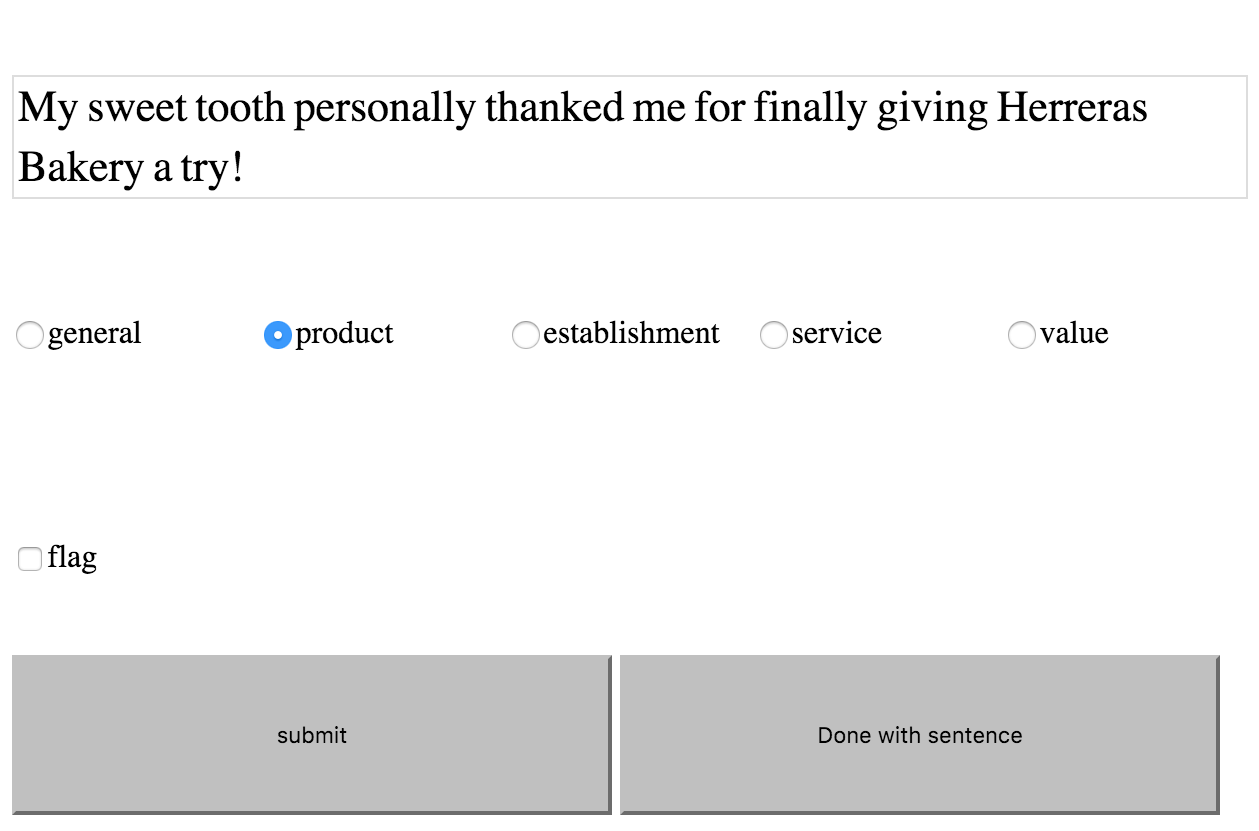
\includegraphics[width=10cm]{annotate_sentence.png}}
  \caption{Sentence level annotation interface}
  \label{fig:annotate_sentence}
\end{figure}

\begin{figure}[h]
  \centering
  \fbox{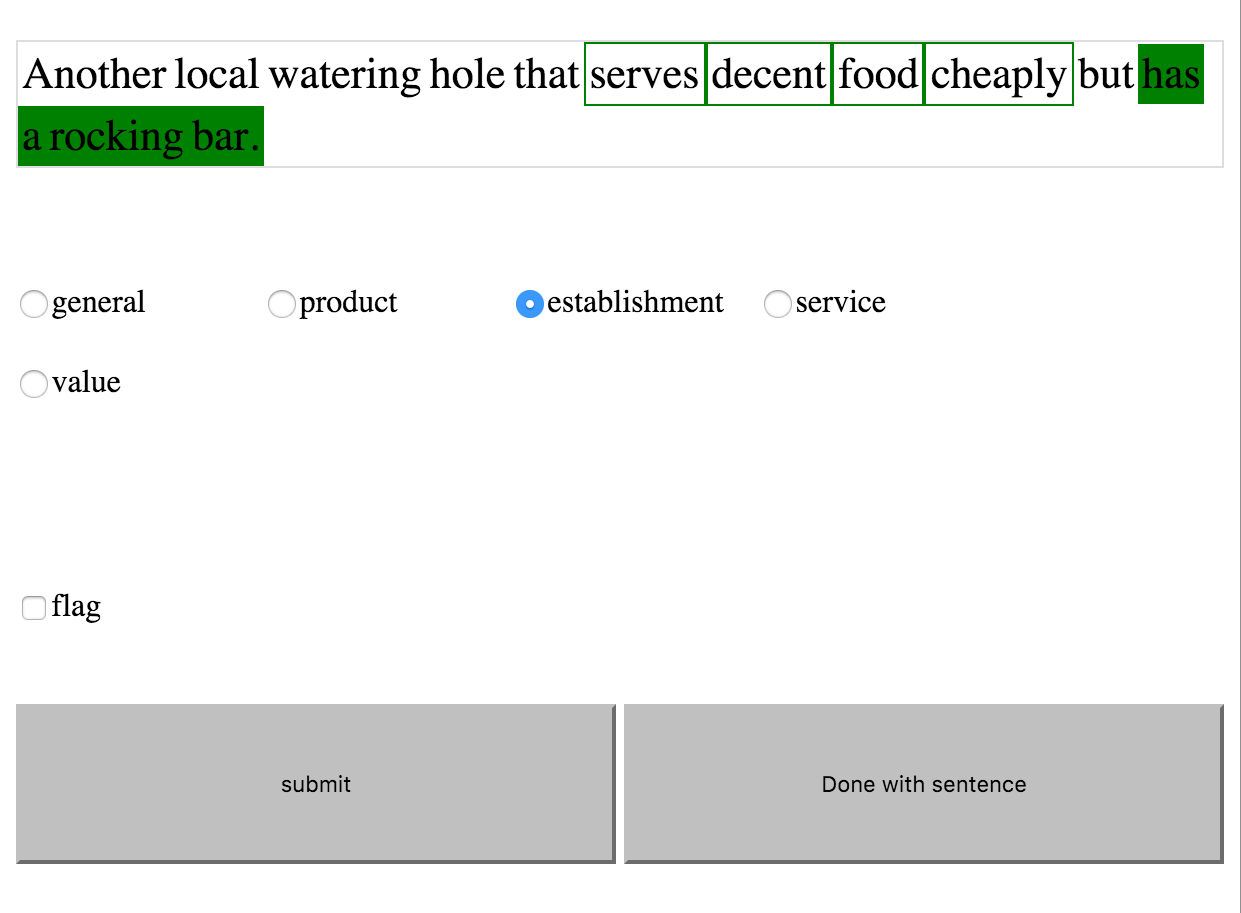
\includegraphics[width=10cm]{annotate_aspect.png}}
  \caption{Aspect level annotation interface. Allowing selection of aspects by marking a series of words(dark green). Since a sentence can hold more than one aspect, once an aspect has been submitted, the same sentence is kept and another aspect can be selected(a green border is left to indicate a previous submission).}
  \label{fig:annotate_aspect}
\end{figure}

Figures \ref{fig:annotate_sentence} and \ref{fig:annotate_aspect} show the interface that was developed to annotate on the \emph{sentence level} and \emph{aspect level} respectively. This simple web-interface was served by a local web server and could be accessed by multiple users simoultaneously.

\newpage

\section{Aspect clustering}
\subsection{Using graph search}
Based on the observation that there is usually some key words in a sentence with lexicographical connection to the desired category, an alternative approach to traditional classification is proposed. This is motivated since classification models need pure training data to achieve good results. The general idea is that using a lexicon of known word relations, one could find a path from a word in a sentence to one of a few labeled word senses, and assign the source word the same label.

Figure~\ref{fig:baklava} shows an example of this premise in action, where the word relations involved in finding the word ``baklava'' were used, and that it is closer to \emph{product} than \emph{establishment}.

\subsection{Basic algorithm}
A \gls{BFS} is conducted from the initial category word senses, defined in table \ref{cat_words}. For each word, neighboring word senses are aquired using word relations defined by \gls{jaws}). Each word sense is also mapped in this process to its source category for future lookups.

Once this ``training phase'' is done, each word in a query sentence is inspected.


\begin{table}[t]
  \centering
  \begin{tabular}{| c | c |}
    \hline
    \textbf{Category} & \textbf{Predefined keywords}\\ \hline
    Establishment & \emph{Furniture, view, music, loud, appearance, clean, location}\\ \hline
    Product & \emph{food, taste, edible}\\ \hline
    Value & \emph{Cheap, price, dollar, buck, lots, happy hour}\\ \hline
    Service & \emph{Service, quick, attentive}\\ \hline
  \end{tabular}
  \caption{Categories with their pre-associated key words.}
  \label{cat_words}
\end{table}

\begin{figure}[t]
  \centering
  \fbox{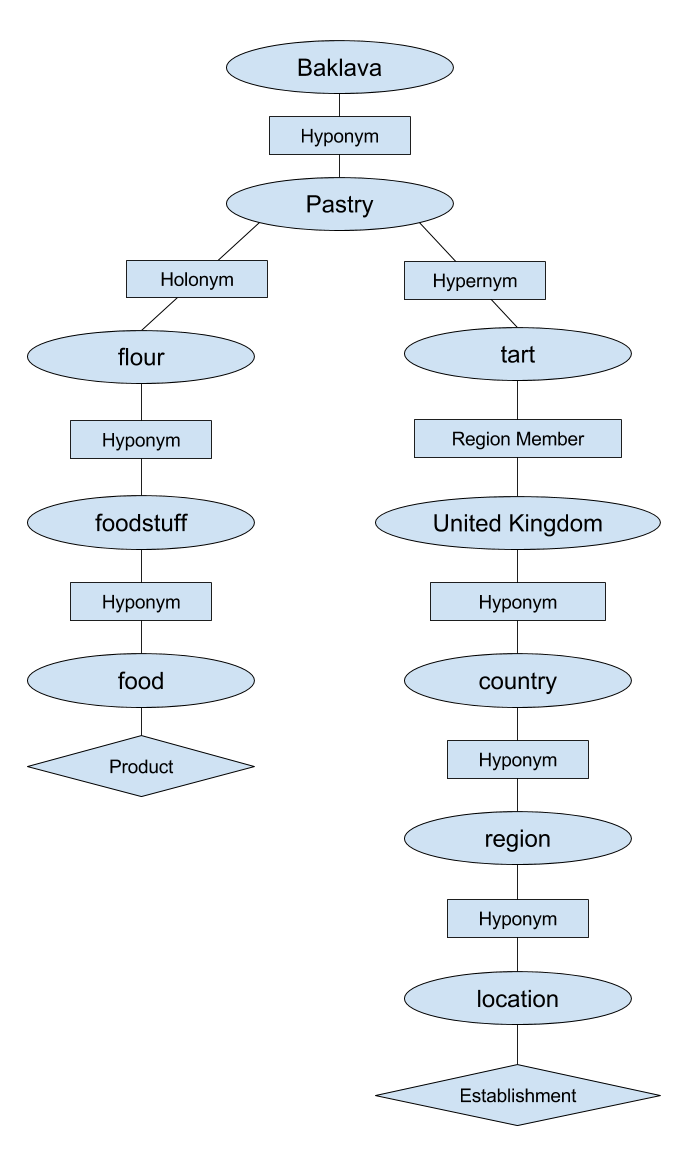
\includegraphics[width=10cm]{img/baklava_lex.png}}
  \caption{Example showing how ``baklava'' could be lexicographically closer to category ``product'' than ``establishment''. Ellipses represent word senses, rectangles the relations between senses, and diamonds predefined categories with a few associated senses (in this case \emph{food} and \emph{location}).}
  \label{fig:baklava_lex}
\end{figure}




% todo: annotations interface screenshot
% todo: num sentences table


\chapter{Results}

This chapter is layed out as follows: First the individual results for each of the \numClassifierAproaches~classifier approaches are walked through. This gives the reader a chance to better understand section \ref{sec:comparison} where the classifiers are compared.


\section{Machine learning classifiers}

\begin{figure}[h!]
  \centering

  \begin{tikzpicture}
    \begin{axis}[
        %title={Classifier performance based on data size},
        xlabel={Training data-set size},
        ylabel={Fraction of correctly classified},
        %xmin=0.3, xmax=0.7,
        %ymin=0.25, ymax=0.75,
        %xtick={0,20,40,60,80,100},
        %ytick={0,20,40,60,80,100,120},
        legend pos=north west,
        ymajorgrids=true,
        grid style=dashed,
      ]
      %\addplot table [x=n, y=p]{data/data_size_unigram.csv};
      \addplot table [x=n, y=p]{data/data_size_unigram_balanced.csv};
      \addplot table [x=n, y=p]{data/data_size_bigram.csv};
      \legend{
        %biased unigram,
        unigram,
        bigram
      }
    \end{axis}
  \end{tikzpicture}
  \caption{Sentence classification performance based on training data size}
  \label{fig:data_size}
\end{figure}


As expected, figure \ref {fig:data_size} shows that increased quantities of training data quickly yield improved results. This increment appears approximately linear, up to some point where it is expected to converge. Interesting is how the simpler unigram method quickly outperforms the bigram model, but that the bigram model sees more promising growth at the cut-off.

\newpage

\subsection{Per class classification}
\begin{figure}[t]
  \centering
  \begin{tikzpicture}

  \begin{axis}[
      %title={Classifier performance per category},
      %xlabel={Categories},
      ylabel={Fraction of correctly classified},
      ybar, ymin=0,
      %bar width=20pt,
      xtick=data,
      x tick label style={rotate=45,anchor=east},
      xticklabels from table={data/per_category_unigram.csv}{n},
      xticklabel style={text height=1.5ex},
      ymajorgrids=true,
      grid style=dashed,
      legend pos=north east,
    ]
    \addplot table [x expr=\coordindex, y=p]{data/per_category_unigram.csv};
    \addplot table [x expr=\coordindex, y=p]{data/per_category_unigram_unbalanced.csv};
    \addplot table [x expr=\coordindex, y=p]{data/per_category_bigram.csv};
    \addplot table [x expr=\coordindex, y=p]{data/per_category_bigram_unbalanced.csv};
    \legend{balanced unigram, unbalanced unigram, balanced bigram, unbalanced bigram}
  \end{axis}
  \end{tikzpicture}
  \caption{Balanced vs. unbalanced classifier comparison. No confidence theshold was set in this experiment: recall was 1.}
  \label{fig:per_cat}
\end{figure}

Section \ref{subsec:bias} introduced bias in data, along with some of its consequences. This motivates a more detailed study of classifier results on a per class basis. Figure \ref{fig:per_cat} illustrates how classifiers trained on balanced training data perfom much more consistent between classes.

Comparison between the balanced/unbalanced versions of the classifier models show that, as expected, there seems to be bias towards the more frequent $product$-class and respectively against the infrequent $value$-class.

It can also be seen that the bigram model is performing poorly for all labels except the \emph{product} class, but the reader is urged to note that this is a consistency between the balanced and unbalanced version of the model.

\newpage

\subsection{Introducing confidence thresholds}
\begin{figure}[t]
  \centering
  \begin{tikzpicture}
    \begin{axis}[
        %title={Classifier performance based on data size},
        xlabel={Recall},
        ylabel={Precision},
        %xmin=0.5, xmax=1,
        %ymin=0.4, ymax=1,
        %xtick={0,20,40,60,80,100},
        %ytick={0,20,40,60,80,100,120},
        legend pos=south west,
        ymajorgrids=true,
        grid style=dashed,
      ]
      \addplot table [x=r, y=p]{data/pr_unigram.csv};
      \addplot table [x=r, y=p]{data/pr_bigram.csv};
      \legend{
        unigram,
        bigram
      }
    \end{axis}
  \end{tikzpicture}
  \caption{Precision vs. recall created varying a confidence threshold}
  \label{fig:pr_curve}
\end{figure}


Figure \ref{fig:pr_curve} shows the expected precision/recall trade-off for the aspect cluster classifiers. Readers should be reminded that each measurement was done on differently balanced training data, which likely accounts for inconsistencies in the curves.

\newpage


\section{Graph-search classifier}
\loremipsum


\section{Comparison of classifiers}
\label{sec:comparison}

\begin{table}[ht]
  \centering
  \pgfplotstabletypeset[
    columns={method,p,r},
    col sep=comma,
    every head row/.style={after row=\midrule},
    columns/method/.style={string type,column type=l, column name=Classifier},
    columns/p/.style={precision=3, column type=l, zerofill, column name=Precision},
    columns/r/.style={precision=4, column type=l, column name=Recall},
  ]{data/general_aspect.csv}

  \vspace{0.4cm}\caption{Result summary}
  \label{general_asp}
\end{table}

\loremipsum
\loremipsum

\pagebreak


\chapter{Discussion}


\loremipsum


\bibliographystyle{plain}
\bibliography{references}

\end{document}
